\chapter{Results and Analysis\label{cha:results_analysis}}
% \ifdraft{In this section you discuss any issues that came up while developing
% the system.  If you found something particularly interesting,
% difficult, or an important learning experience, put it here.  This is
% also a good place to put additional figures and data.}{}

The results chapter deals with presenting the different metrics discussed so far, within the RECAT-EU scheme. The data subset for the analysis was limited to four pair categories from the ICAO scheme: H-H, H-M, M-H, M-M. This simplification was done in order to filter out the small number of data points for the other pairs, insufficient for any valid estimations. 

Each of the ICAO pairs were re-categorised, the data-set was reduced once more, again filtering out the pair categories with insufficient number of data points. 
The distribution of inter-arrival distances for the RECAT-EU pairs were examined in agreement with the RECAT-EU reference separations. The LTI and AROT for particular pairs were compared to identify the limiting factor for throughput capacity, using the method already introduced in section \ref{ssec:LTI}.

% Please add the following required packages to your document preamble:
% \usepackage{multirow}
% \usepackage{graphicx}
% \usepackage[table,xcdraw]{xcolor}
% If you use beamer only pass "xcolor=table" option, i.e. \documentclass[xcolor=table]{beamer}
\begin{table}[h]
\centering
\resizebox{0.8\textwidth}{!}{%
\begin{tabular}{cc|c|c|c|c|c|c|}
\cline{3-8}
\multicolumn{1}{l}{} & \multicolumn{1}{l|}{} & \multicolumn{6}{c|}{Follower} \\ \cline{3-8} 
\multicolumn{1}{l}{} & \multicolumn{1}{l|}{} & CAT-A & CAT-B & CAT-C & CAT-D & CAT-E & CAT-F \\ \hline
\multicolumn{1}{|c|}{} & CAT-A &  &  &  & \cellcolor[HTML]{FFFFC7}1 &  &  \\ \cline{2-8} 
\multicolumn{1}{|c|}{} & CAT-B &  & \cellcolor[HTML]{FFFFC7}1 & \cellcolor[HTML]{FFFC9E}17 & \cellcolor[HTML]{FFFC9E}16 & \cellcolor[HTML]{FFFFC7}2 &  \\ \cline{2-8} 
\multicolumn{1}{|c|}{} & CAT-C &  & \cellcolor[HTML]{FFFC9E}19 & \cellcolor[HTML]{FD6864}1697 & \cellcolor[HTML]{FE996B}242 & \cellcolor[HTML]{FFCE93}41 & \cellcolor[HTML]{FFFC9E}14 \\ \cline{2-8} 
\multicolumn{1}{|c|}{} & CAT-D & \cellcolor[HTML]{FFFFC7}1 & \cellcolor[HTML]{FFFC9E}10 & \cellcolor[HTML]{FE996B}229 & \cellcolor[HTML]{FE996B}200 & \cellcolor[HTML]{FFFC9E}10 & \cellcolor[HTML]{FFFFC7}5 \\ \cline{2-8} 
\multicolumn{1}{|c|}{} & CAT-E &  & \cellcolor[HTML]{FFFFC7}1 & \cellcolor[HTML]{FFCE93}44 & \cellcolor[HTML]{FFFFC7}10 &  &  \\ \cline{2-8} 
\multicolumn{1}{|c|}{\multirow{-6}{*}{\rotatebox[origin=c]{90}{Leader}}} & CAT-F &  &  & \cellcolor[HTML]{FFFC9E}16 & \cellcolor[HTML]{FFFFC7}10 & \cellcolor[HTML]{FFFFC7}1 &  \\ \hline
\end{tabular}%
}
\caption[BIKF traffic mix sorted into RECAT-EU categories]{Number of RECAT-EU pairs from the traffic mix at BIKF during peak hours, arranged into the corresponding wake categories. The majority of arrival pairs are classified as C-C. The observation period is from October 2017 to November 2018.}
\label{tab:pairs_mix_to_recat}
\end{table}

\section{Inter-arrival Distance Separation of RECAT-EU pairs}\label{sec:interarrival_dist_sep_RECAT}
The mix of arrival pairs from the peak hour traffic at BIKF after re-categorisation are presented in Table~\ref{tab:pairs_mix_to_recat}. As expected from the traffic fleet analysis in \ref{ssec:traffic_mix}, most of the aircraft combined into C-C pairs. The rest of the more significant traffic pairs were variations from CAT-C, CAT-D and CAT-E categories.\\
The resulting pairs from the ICAO H-H pairs were re-categorised primarily as C-C (87,5\%) and C-B (10,7\%) into the RECAT-EU scheme (Table~\ref{fig:HH_to_RECAT_pairs_dist_separ}). It is apparent that for those pairs the RECAT-EU scheme would decrease the required separation minima by one nautical mile (from 4 NM to 3 NM). The share of the H-H pairs was 2,2\% of all observed pairs at BIKF.

\begin{figure}[h]
    \centering
    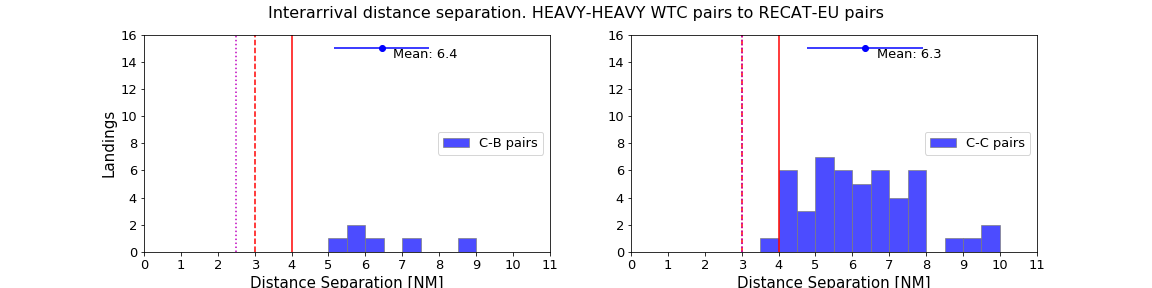
\includegraphics[width=1\textwidth]{graphics/fig_HH_to_RECAT_pairs_dist_separ.png}
    \caption[Inter-arrival distance separation of ICAO H-H pairs into the RECAT-EU scheme]{Inter-arrival distance separation after re-categorisation of ICAO H-H pairs into the RECAT-EU scheme. The vertical lines indicate the separation minima in different schemes (ICAO - solid red line, RECAT-EU - dashed red line, MRS - dotted magenta line)}
    \label{fig:HH_to_RECAT_pairs_dist_separ}
\end{figure}

For the aircraft pairs of the ICAO H-M category the transition to the RECAT-EU scheme will decrease the separation minima requirements more noticeably. The reduction for aircraft pairs that were re-categorised as B-C or B-D category is from 5 NM to 4 NM, while for the C-C and C-D pairs this reduction is 2~NM, from 5~NM to 3~NM (Figure~\ref{fig:HM_to_RECAT_pairs_dist_separ}). Here again the C-C pairs were predominant with 73,8\% and C-D pairs with 10,8\%. The share of the B-C and B-D pairs was around 5\%. Provided that the MRS requirements allow for reduced minima, the D-D pairs from the ICAO H-M pair category would have potentially 2,5~NM reduction, but only three of those pairs were present in the observed data subset (Figure~\ref{fig:HM_to_DD_pairs_dist_separ}). The share of the H-M pair category from the whole BIKF traffic during peak hours is 12,9\%.

\begin{figure}[h]
    \centering
    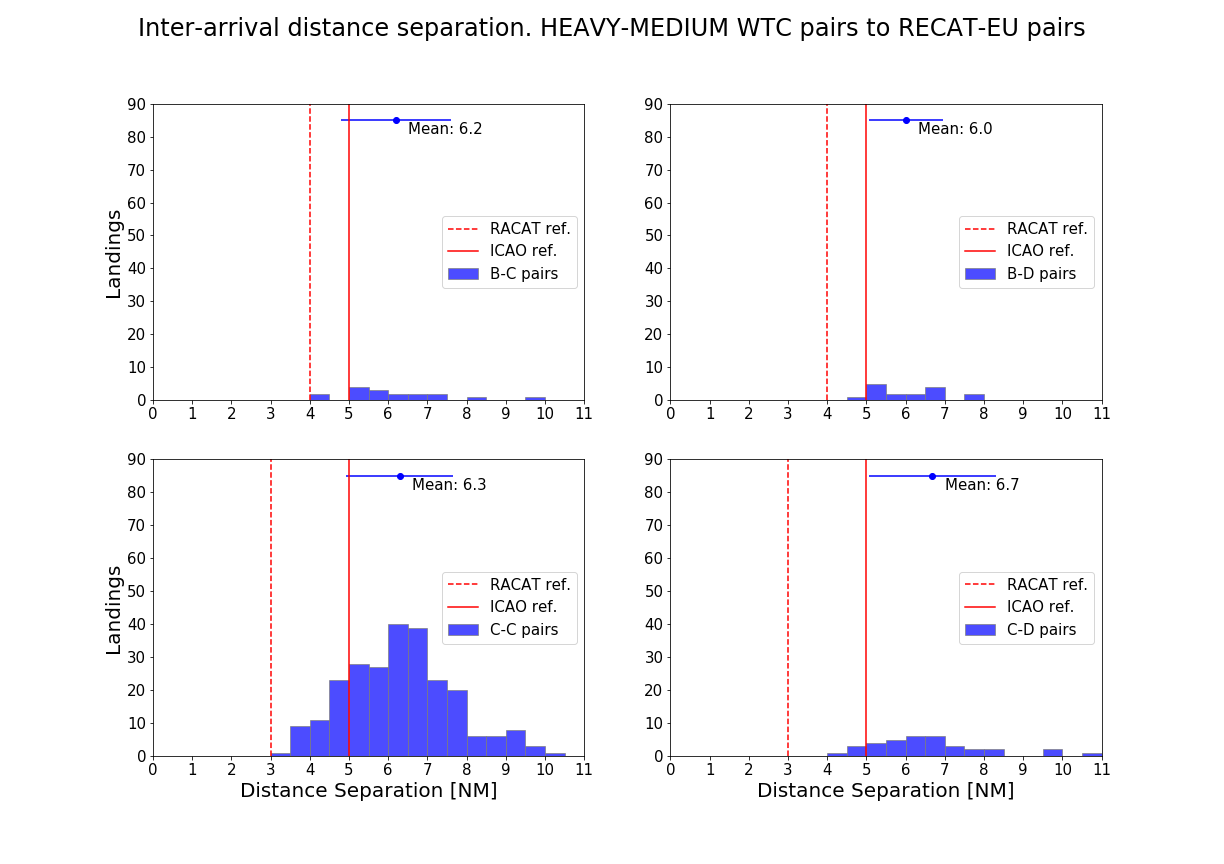
\includegraphics[width=1\textwidth]{graphics/fig_HM_to_RECAT_pairs_dist_separ.png}
    \caption[Inter-arrival distance separation of ICAO H-M pairs into the RECAT-EU scheme]{Inter-arrival distance separation after re-categorisation of ICAO H-M pairs into the RECAT-EU scheme.}
    \label{fig:HM_to_RECAT_pairs_dist_separ}
\end{figure}

The re-categorisation of  the ICAO M-H (Figure~\ref{fig:MH_to_RECAT_pairs_dist_separ}) and M-M (Figure~\ref{fig:MM_to_RECAT_pairs_dist_separ}) pairs from the data subset shows no apparent advantage for the newly formed RECAT-EU pairs. The traffic in both cases is concentrated in the C-C pairs category. The RECAT-EU reference separation minima does not change its position after re-categorisation to allow for any shift in the separation distribution between aircraft pairs. In both schemes the reference separation was specified as 3 NM, or 2,5 NM when the MRS was applicable. In the case of BIKF the MRS minima was established at 3 NM because of technical characteristics of the radar system, as mentioned earlier. The 2,5 NM dotted line in the figures was drawn just for comparison and not as a reference minima limit.  Pairs from the C-C category comprise 77,9\% of all the ICAO M-H pairs, followed by the D-C pair category with 11,4\%.

\begin{figure}[h]
    \centering
    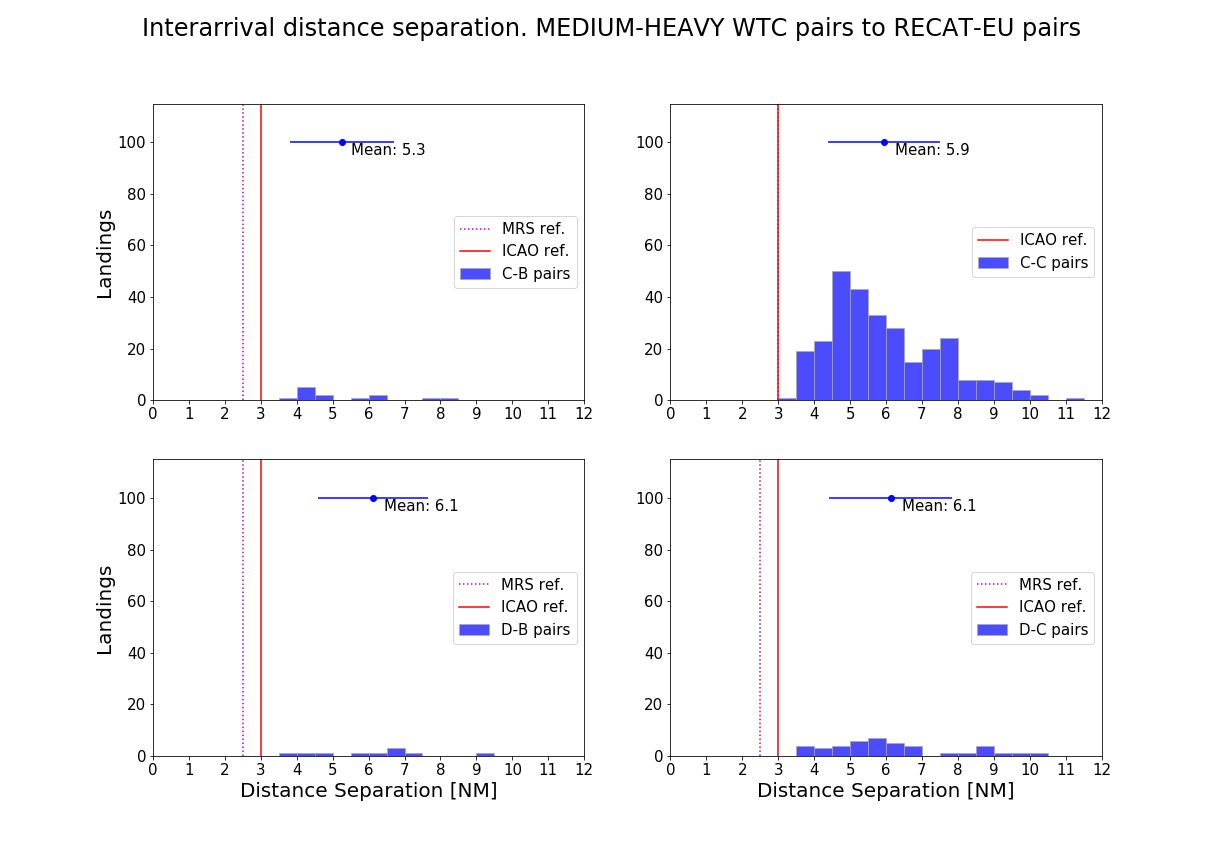
\includegraphics[width=1\textwidth]{graphics/fig_MH_to_RECAT_pairs_dist_separ.png}
    \caption[Inter-arrival distance separation of ICAO M-H pairs into the RECAT-EU scheme]{Inter-arrival distance separation after re-categorisation of ICAO M-H pairs into the RECAT-EU scheme.}
    \label{fig:MH_to_RECAT_pairs_dist_separ}
\end{figure}

The portion of C-C pairs from the last category, the M-M pairs, is also prevailing with 61,8\%, followed by the C-D (11,4\%), D-D (10,8\%) and D-C (10,4\%) pairs. The lower percentage of the C-C pairs from the ICAO M-M category in comparison with the other ICAO categories after re-categorisation was accompanied by increased ratio of the other pair categories, as noticed in the percentage values and in Figure~\ref{fig:MM_to_RECAT_pairs_dist_separ}. The reference separation minima remains unchanged after re-categorisation, similar to the M-H pairs. This result was also evidence that most of the aircraft traffic mix for Keflavík Airport were in the Medium category.

\begin{figure}[h]
    \centering
    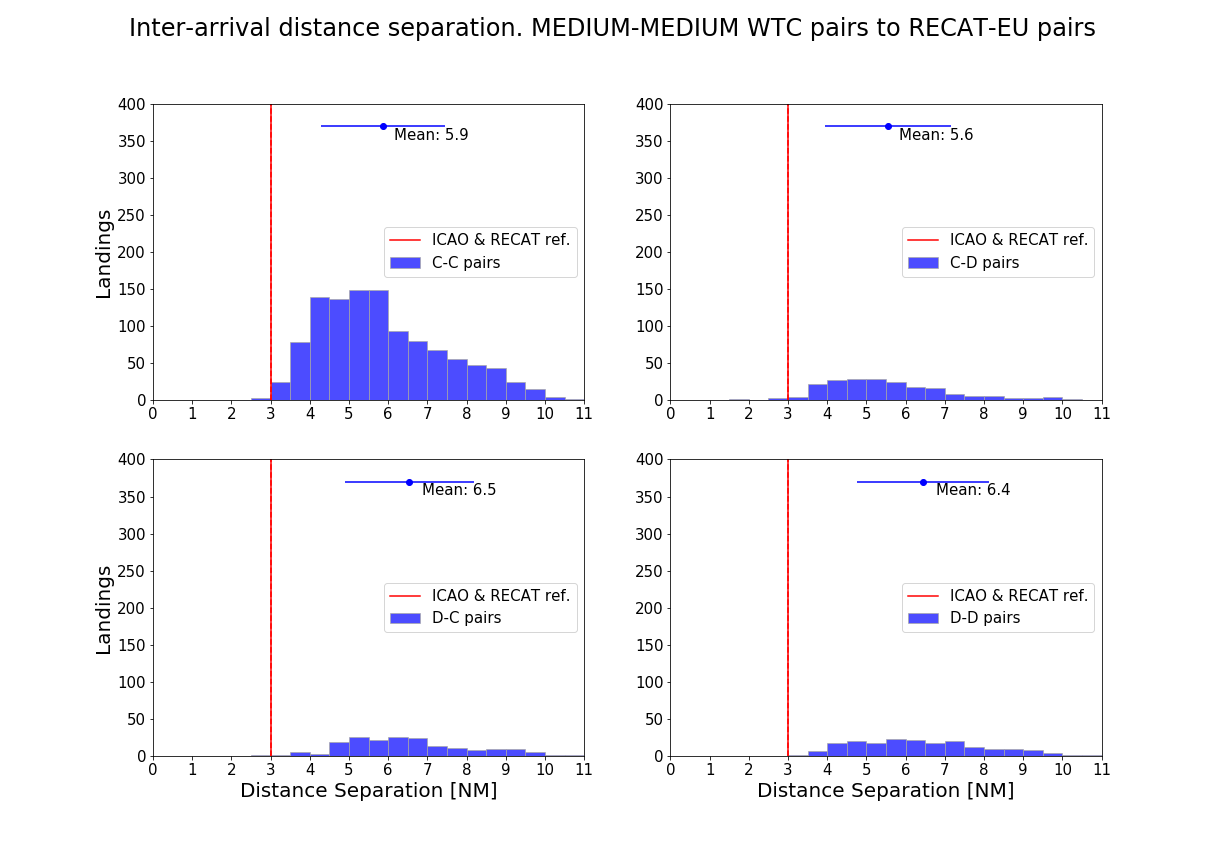
\includegraphics[width=1.0\textwidth]{graphics/fig_MM_to_RECAT_pairs_dist_separ.png}
    \caption[Inter-arrival distance separation of ICAO M-M pairs into the RECAT-EU scheme]{Inter-arrival distance separation after re-categorisation of ICAO M-M pairs into the RECAT-EU scheme.}
    \label{fig:MM_to_RECAT_pairs_dist_separ}
\end{figure}

The share of the M-H pairs from the whole BIKF traffic during peak hours is 14,3\%. The share of the M-M pairs on the other hand is the largest of all ICAO pairs - 69.8\%. The figures above were also evidence that incorporating the RECAT-EU scheme for the selected data subset, would potentially assist the aircraft pairs with a Heavy leader, but would not change the situation for pairs with a Medium leader. 

It is illustrative to mention also that some of the pair categories would suffer an increase in the separation minima in the RECAT-EU scheme. Such example from the traffic at Keflavík would be the C-F and D-F pairs from the ICAO M-M category (Figure~\ref{fig:MM_to_CF_and_DF_pairs_dist_separ}). The reference separation in the former case would double from 3 NM up to 6 NM and in the later case the increase would be from 3 NM to 5 NM. Those pairs were rare in the data set and insufficient to reach any accurate conclusion. Only two pairs from the M-M category for the selected time period were in the D-F category and eight pairs were in the C-F category.

\begin{figure}[h]
    \centering
    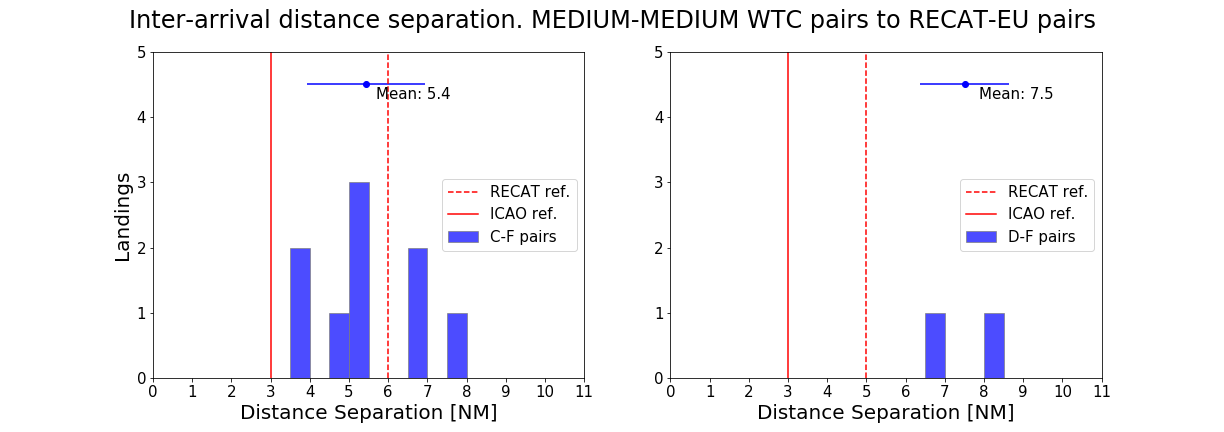
\includegraphics[width=1\textwidth]{graphics/fig_MM_to_CF_and_DF_pairs_dist_separ.png}
    \caption[Inter-arrival distance separation of ICAO M-M pairs into the RECAT-EU C-F and D-F pairs]{Inter-arrival distance separation after re-categorisation of ICAO M-M pairs into the RECAT-EU C-F and D-F pairs.}
    \label{fig:MM_to_CF_and_DF_pairs_dist_separ}
\end{figure}


\section{Runway Occupancy and Landing Time Interval for RECAT-EU pairs}
The following section presents the landing time intervals (LTI) for a subset of data points after re-categorisation from the ICAO wake turbulence scheme. The subset contained primarily C-C pairs. The C-C pairs were selected on the basis of being the more prominent subset with most of the data points. The LTI for the ICAO pair sets from \ref{ssec:LTI} were modified to represent only the C-C pairs, where the effect on the LTI distribution after re-categorisation would be more accurate. The other metric used in contrast to the LTI was the arrival runway occupancy time for the respective aircraft pairs. The frequency distribution of the AROT included the runway occupancy for all the leaders of the selected ICAO category in order to make use of more data points and obtain a more general view on the AROT distribution. This decision was based on the assumption that the AROT of the leader in an aircraft pair is the constraint for the time separation of follower. This is illustrated in the result for the LTI and the AROT for the C-C pairs from H-H pair category in Figure~\ref{fig:CC_from_HH_pairs_time_sep}. 

\begin{figure}[h]
    \centering
    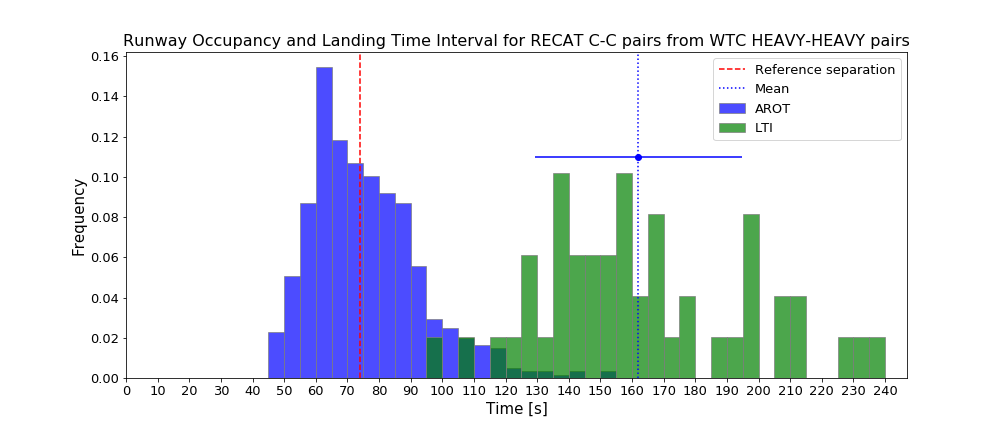
\includegraphics[width=1\textwidth]{graphics/fig_CC_from_HH_pairs_time_sep.png}
    \caption[AROT and LTI of C-C pairs originating from ICAO H-H pairs]{AROT and landing time intervals of C-C pairs originating from ICAO H-H pairs. The dashed red line indicates the RECAT-EU reference time separation for the C-C pairs.}
    \label{fig:CC_from_HH_pairs_time_sep}
\end{figure}

The LTI frequency distribution contained all C-C pairs originating from the ICAO H-H category. The reference time separation (red dashed line) was calculated from the final approach speed and the RECAT-EU distance separation, as explained in \ref{ssec:LTI}. The frequency distribution for the AROT, on the other hand, contained all pairs with CAT-C leader originating from the Heavy category, not only pairs with CAT-C leader and CAT-C follower. In this sense the distribution for the AROT was based on more data points than the distribution for the LTI and gave a more accurate presentation of the runway occupancy. Figure~\ref{fig:CC_from_HH_pairs_time_sep} represents the case for 1,9\% of all arrival pairs at BIKF for the observed period during peak hours.

The share of C-C pairs originating from the ICAO H-M category from the peak traffic at the airport was 9,5\%.  The LTI frequency distribution of those pairs is shown in Figure~\ref{fig:CC_from_HM_pairs_time_sep}. Here again the AROT distribution was based on the runway occupancy of CAT-C leaders, as in the previous case. 
 
\begin{figure}[h]
    \centering
    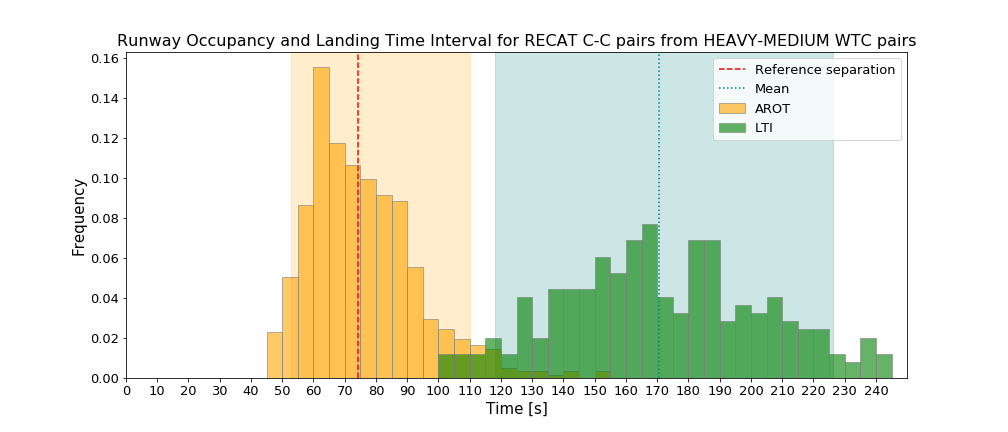
\includegraphics[width=1\textwidth]{graphics/fig_CC_from_HM_pairs_time_sep.png}
    \caption[AROT and LTI of C-C pairs originating from ICAO H-M pairs]{AROT and landing time intervals of C-C pairs originating from ICAO H-M pairs. The dashed red line indicates the RECAT-EU reference time separation for the C-C pairs.}
    \label{fig:CC_from_HM_pairs_time_sep}
\end{figure}

These two cases: C-C pairs from ICAO H-H and H-M categories, would have more noticeable beneficial effect from the implementation of the RECAT-EU scheme (refer to~\ref{sec:interarrival_dist_sep_RECAT}). The decrease in distance separation in those cases is 1 NM or 2 NM. Translating the separation into the time domain resulted in a separation reference time line at 74 seconds and minimum LTI values close to 100 seconds. This shift of the reference line creates the potential for shift to the left in the frequency distribution of the LTI.
 
 \begin{figure}[h]
    \centering
    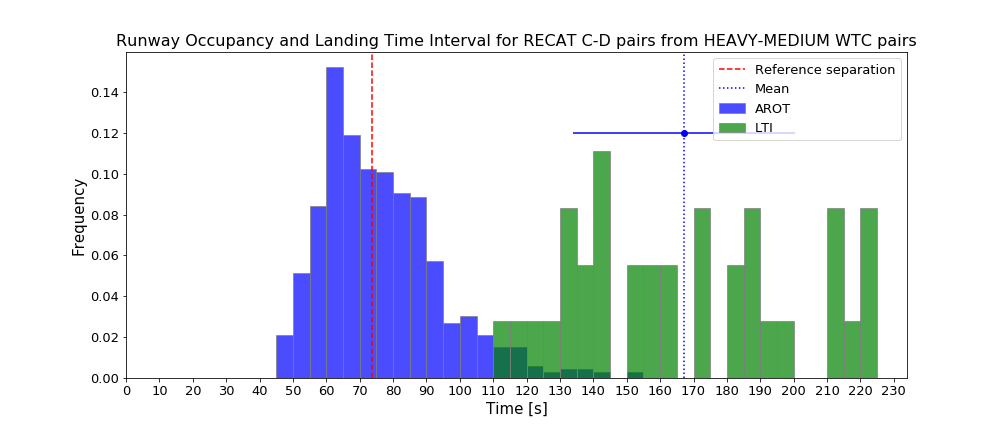
\includegraphics[width=1\textwidth]{graphics/fig_CD_from_HM_pairs_time_sep.png}
    \caption[AROT and LTI of C-D pairs originating from ICAO H-M pairs]{AROT and landing time intervals of C-D pairs originating from ICAO H-M pairs. The dashed red line indicates the RECAT-EU reference time separation for the C-D pairs.}
    \label{fig:CD_from_HM_pairs_time_sep}
\end{figure}

Even greater potential for decrease of the inter-arrival time was observed in the case of C-D pairs from the ICAO H-M category (Figure~\ref{fig:CD_from_HM_pairs_time_sep}). Here the minimum LTI observed was 113 seconds, serving as a possible 39 seconds shift to the left of the frequency distribution. However the share of those pairs in the traffic was limited to 1.4\%.

The C-C pairs formed from the ICAO M-H category were 11,1\% from the BIKF traffic with frequency distribution of the LTI shown in Figure~\ref{fig:CC_from_MH_pairs_time_sep}. The reference line in this case is again at 74 seconds, and the LTI frequency distribution curve was closer to the reference than in the cases above.

\begin{figure}[h]
    \centering
    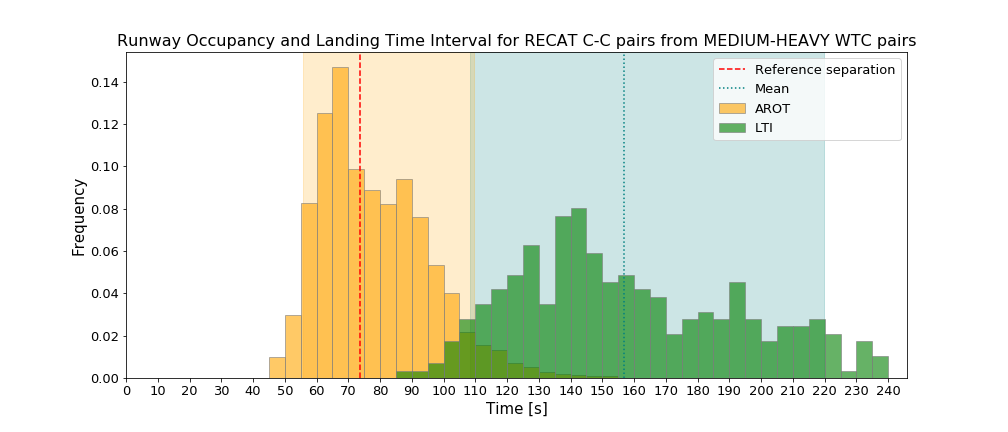
\includegraphics[width=1\textwidth]{graphics/fig_CC_from_MH_pairs_time_sep.png}
    \caption[AROT and LTI of C-C pairs originating from ICAO M-H pairs]{AROT and landing time intervals of C-C pairs originating from ICAO M-H pairs. The dashed red line indicates the RECAT-EU reference time separation for the C-C pairs.}
    \label{fig:CC_from_MH_pairs_time_sep}
\end{figure}

The majority of the C-C pairs of the BIKF traffic were formed from the ICAO M-M pairs, or 43\%. Here the minimum inter-arrival time separation was 80 seconds, a mere 6 seconds above the reference limit, with half of all pairs having LTI between 132 and 185 seconds.

\begin{figure}[h]
    \centering
    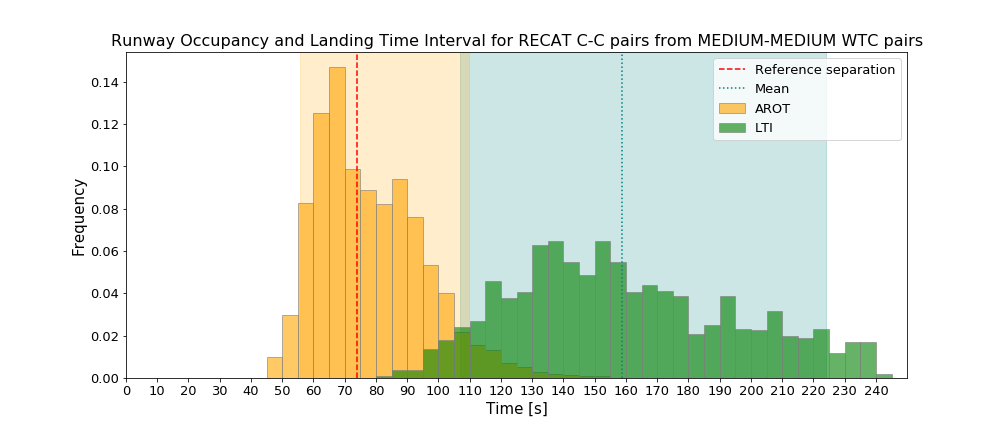
\includegraphics[width=1\textwidth]{graphics/fig_CC_from_MM_pairs_time_sep.png}
    \caption[AROT and LTI of C-C pairs originating from ICAO M-M pairs]{AROT and landing time intervals of C-C pairs originating from ICAO M-M pairs. The dashed red line indicates the RECAT-EU reference time separation for the C-C pairs.}
    \label{fig:CC_from_MM_pairs_time_sep}
\end{figure}

Nevertheless the potential for decrease of the landing time interval was hindered by the AROT, the other major factor affecting runway capacity (refer to \ref{sec:runway_capacity}). All of the distributions in the figures above witness an overlap of the reference time separation line and the AROT frequency distribution. The average runway occupancy time was estimated as 77,5 seconds (\ref{sssec:runway_usage_arot}) and compared to the reference time line for the predominant C-C pairs (74 seconds), it is apparent that the AROT is the limiting factor and a major constraint for shift in the LTI distribution.








% \lipsum[28-34]

%%% Local Variables: 
%%% mode: latex
%%% TeX-master: "DEGREE-NAME-YEAR"
%%% End: 
